\chapter{PHILOSOPHIE DU DESIGN--INDUSTRIEL DE YEROTH--ERP--$3.0$}


\begin{center}
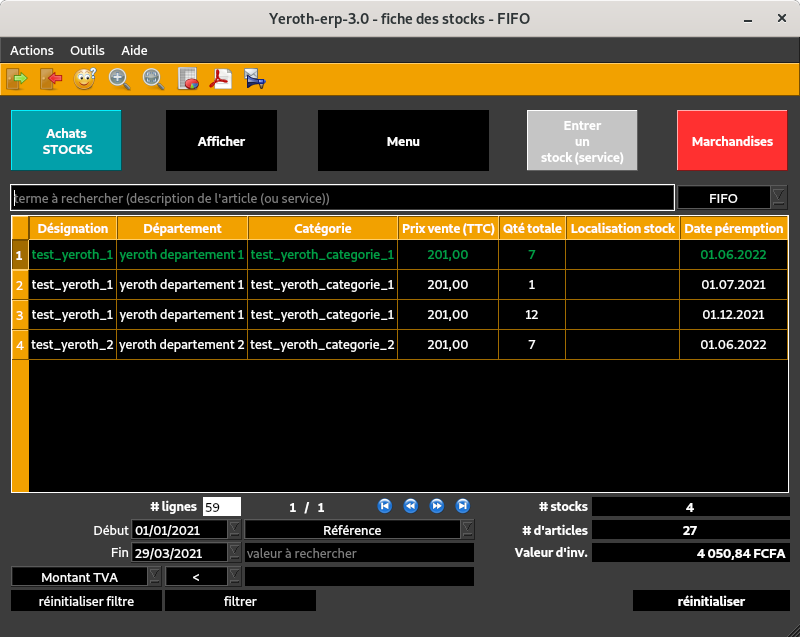
\includegraphics[scale=0.52]{images/yeroth-erp-3-0-stocks-fenetre-screenshot.png}
\captionof{figure}{La fen\^etre de visualisation de stocks.}
\label{fig:fenetre-de-visualisation-de-stocks-DESIGN_YEROTH_ERP_3_0}
\end{center}


J'AI CONSTRUIT ET IMPLÉMEMTÉ \yerotherpblack AVEC LES OBJECTIFS
SUIVANTS:

\begin{enumerate}[1.]
	\itemsep 0.75em

	\item \yerothpurplishbf{Les champs de texte destinés
		à la recherche textuelle arbore dans leur espace
		d'écriture, des indications sur la fiabilité et
		la pertinence des résultats}.
		
		cf. l'image de la fenetre~\ref{fig:fenetre-de-visualisation-de-stocks-DESIGN_YEROTH_ERP_3_0}
		de visualition des stocks de \yerotherpblack; 
		le champs textuel juste en-dessous du BOUTON 'menu'
		mentionne que toute recherche effectuée en son sein,
		se fera uniquement dans la COLONE 'DESCRIPTION DE
		L'ARTICLE, OU DU SERVICE'.
	
	\item \yerothpurplishbf{\yerotherpblack est privé en presque
		tout point de la MAXIMISATION DES FENÊTRES:
		CECI DANS LE SOUCIS DE POUVOIR UTILISER \yerotherpblack}.
		
	\item \yerothpurplishbf{\yerotherpblack est portable:
		\begin{enumerate}[1.]
			\item sur toutes les plateformes possible ayant
				juste $1$ compilateur \cplusplus
			\item (ANDROID--GOOGLE) grâce l'outil
			\qtcreator.
		\end{enumerate}}

	\item \yerothpurplishbf{L'utilisateur a accès en tout
		point du logiciel à $1$ autre en exécutant au
		GRAND MAXIMUM \textbf{$3$ actions}}: \textbf{RÈGLE DE $3$ CLICKS}.

\end{enumerate}
